\documentclass[12pt]{report}
\usepackage[margin=2cm, left=3cm, top=2cm, bottom = 2cm]{geometry} % set margins
\usepackage{times}
\usepackage{setspace} % for line spacing
\usepackage{amsmath}
\usepackage[authordate]{biblatex-chicago}
\usepackage{sidenotes}
\usepackage{microtype}
\usepackage{siunitx}
\usepackage{titlesec}
\usepackage{pgfplots}
\usepackage{longtable}
\usepackage{tabularx}
\usepackage{multirow}
\usepackage{fancyhdr}
\usepackage{booktabs}
\usepackage{siunitx}
\usepackage{footmisc} % for footnote size
\pgfplotsset{compat=1.16}

\titleformat{\section}
  {\normalfont\Large\bfseries} % format
  {\thesection.} % label
  {1em} % sep
  {} % before-code
\renewcommand{\thesection}{\arabic{section}}
\newcommand{\percent}{\%}
\setlength{\headheight}{15pt}
\pagestyle{fancy}
\fancyhf{} % clear all header and footer fields
\fancyhead[L]{Maxim Efimov}
\fancyfoot[L]{\today}
\fancyfoot[R]{Page \thepage}

\addbibresource{Thesis.bib}

\title{Predicting real estate prices: Comparing traditional and machine learning methods}
\author{Maxim Efimov}
\date{\today}

\begin{document}
\pagenumbering{gobble} % turn off page numbering
\maketitle
\tableofcontents
\newpage
\pagenumbering{arabic} % turn on page numbering
\setstretch{1.5} % set line spacing
\fontsize{12}{18}\selectfont % set font size
\renewcommand{\footnotesize}{\fontsize{10}{12}\selectfont} % set footnote size


\newpage

\section{Introduction}
\subsection{Background}

Real estate markets are as old as the human civilisation itself, but with new technological advancements they were able to become more open and transparent, more standardised and sophisticated than ever. Modern rental and house sale listing websites include a vast variety of metrics, from internal, propriety metrics like the Zillow price estimation score “Zestimate”, to third-party metrics like the “walkability score”, to landlord- and tenant-submitted information like the exact contract details and unit features. At the same time, the manifold increases in semiconductors’ computational power, as well as the gradual improvements in data analyses algorithms allow us to analyse the data in more sophisticated ways, untangling at times non-linear relations or non-obvious interactions between variables.
\subsection{Literature Review}

With these technological advancements, it is pertinent to see what type of algorithm is better suited for taking a variety of metrics regarding a given housing unit and predicting its rental costs. The current research is extensive when it comes to use of modern advanced regression techniques on both rental (\cite{neloy2019}) and home-buying (\cite{Shahhosseini2001}) prices. At the same time, existing models rarely if ever take advantage of the abundance of the modern data, focusing instead on a relatively small number of core characteristics (e.g. square footage, distance from the centre).

\subsection{Aim and research questions}

The goals of this paper then will be to see if the neighbourhood-related data points provided on modern real estate digital platforms provide a significant amount of extra goodness of fit, and whether the more complicated to use, more computationally intense algorithms provide better analysis of voluminous, complicated data with gaps, large potential for non-linear relations and hard-to interpret coefficients. The paper will consist of answering two research questions: “Do neighbourhood characteristics reliably influence the rental price of housing units?”  with the expectation that they do, and “Which econometric prediction model uses a variety of provided data to create a prediction model with the best goodness-of-fit score?”, where the expectation is that the neural network will be best suited to make predictions based on the data, due to it being the most computationally expensive, most ``open-minded" model, able to operate with a lot fewer assumptions about the underlying data, than the other two. Goodness of fit will be evaluated using $R_adjusted^2$ - the adjustment is necessary, since the models with and without the neighborhood dummy-variables will have a drastically different number of variables, and so due to the variance-bias tradeoff, the un-adjusted $R^2$ will always be larger in a model with more parameters.

This thesis can provide value by showcasing the strengths and weaknesses of each method and finding out what is the best method for analysis on both the platform, the landlord and the prospective tenant’s side – that is to say, what method one should use to compare a given rental unit against others in the same area.

\section{Data}

\subsection{Data sources}

For this work, data from the Zillow rental database for the Chicago area will be used. The full dataset on Zillow includes around 6000 listings, with the precise number varying depending on day and season of the year. Zillow was chosen due to the availability of its data and the high amount of data points available for each listing, including some that are calculated by the website itself. The dataset is not without its flaws, however -- due to the website managers' anti-AWI\footnote{Automated Web Interactors} policy, collecting the entire database proved perilous. In the end, a representative sample was chosen -- it consists of random houses, chosen proportionally from each rental price bracket -- see Figures 1 and 2 for comparison between the rent distribution of the dataset and the sample. Note that listings with rental prices below \$600 were excluded, since despite nominally making up a sizeable part of the overall data, they in practice consist mostly of listings with unspecified rent price.
As we can see in figures \ref{fig:plot1} and \ref{fig:plot2}, the distribution of the sample is relatively similar to that of the overall dataset, and so it can be considered representative.

\begin{figure}[h!]
	\begin{minipage}{0.5\textwidth}
		\begin{tikzpicture}
			\begin{axis}[
					ybar,
					xtick=data,
					xticklabel style={rotate=270},
					xticklabels = {},
					xlabel={Rental Unit Price, USD},
					xlabel style={at={(axis description cs:0.5,-0.001)},anchor=north},
					ylabel={Listings, N},
					name=plot1,
					at={(0,0)},
					anchor=south west,
					scale only axis,
					width=0.8\textwidth,
					height=0.3\textheight
				]
				\addplot+ coordinates {(0,57) (1,287) (2,496) (3,861) (4,814) (5,790) (6,852) (7,658) (8,688) (9,576) (10,465) (11,368) (12,273) (13,240) (14,233) (15,198) (16,159) (17, 111)};
			\end{axis}
		\end{tikzpicture}
		\caption{Distribution of rental units on the \\ Zillow online repository}
		\label{fig:plot1}
	\end{minipage} % < -- this comment ensures that there is no line break between the minipages
	\begin{minipage}{0.5\textwidth}
		\begin{tikzpicture}
			\begin{axis}[
					ybar,
					xtick=data,
					xticklabel style={rotate=270},
					xticklabels ={},
					xlabel={Rental Unit Price, USD},
					xlabel style={at={(axis description cs:0.5,-0.001)},anchor=north},
					ylabel={Listings, N},
					at = {(0,0)},
					anchor=south west,
					scale only axis,
					width=0.8\textwidth,
					height=0.3\textheight
				]
				\addplot+ coordinates {(0,18) (1,140) (2,235) (3,463) (4,618) (5,491) (6,620) (7,588) (8,518) (9,561) (10,316) (11,156) (12,91) (13,82) (14,120) (15,114) (16, 100) (17, 71)};
			\end{axis}
		\end{tikzpicture}
		\caption{Distribution of rental units in the sample \\}
		\label{fig:plot2}
	\end{minipage}
\end{figure}

\subsection{Data acquisition}
Data was acquired from the Zillow website using AWI techniques with the help of a browser extension called ``webscraper.io". The extension allows the user to select the desired data on the website, and then automatically scrape it into a .csv file. The data was then cleaned and processed using the Python 3.11 programming language. The code used for data acquisition and cleaning is available in the appendix. This tool, however, has its limitations -- sometimes, other data from unrelated listings -- most notably, houses for sale, rather than rent -- and have to be removed later. It also does not always capture commute values of apartment complexes with multiple listings -- those values will then have to be imputed -- nor does it always copy information of every listing on the website - for a comparison of distributions of listings' rent prices in the dataset and the sample, see Figures 1 \& 2. For other information, such as 'facts and features', the extension creates a single unpunctuated text block, which has to be further parsed with the use of Python and regular expressions. Luckily, Zillow stores the data using a standardised format, making it simple to look for specific words and expressions, always appearing in the same place and phrased the same way for all listings.

\subsection{Data description}

The resulting sample consists of N listings, each with 60 variables. The list of variables is given in Figure 3. ``Commute" here means a metric, provided by Zillow itself -- the platform allows its users to select one or several places of their current work, and the platform then plots the most efficient course for the chosen method of transportation between the unit selected and those places. This metric was used as a potentially superior and more convenient alternative to distance from the centre of the city, since it takes into consideration how traffic density and ease of transportation can affect from equidistant points. For the sake of this paper, Willis Tower was chosen as a commute point -- this building is both the most well-known and tallest in Chicago, and is located in the very centre of the city's office district, the Loop. Thus, it can act as a proxy for the city centre and work commute location of most renters. Categorical variables, such as flooring, allowed pets and others, were separated into boolean ``dummy" variables.

\subsection{Data cleaning}
During the cleaning process, listings with unstated rental price or square footage were removed. Crime rates were extrapolated from neighbourhood-wide data, provided on the website ``Neighbourhood Scout", which collects its data from U.S. law enforcement agencies. Missing values were imputed, with imputation methods differing by column, giving preference to more precise methods of imputation if possible. For instance, while the missing values in the columns ``footageplural" and ``arrests" were filled with the sample and city mean, school rating data was filled with the mean of other, non-missing school ratings, deposits and application fees were filled with the average for the units from the same rent bracket, since many flats' deposits and fees are set to be multiples of monthly rent. Area-specific variables, such as commute time, were first imputed based on the units' postcodes, then based on the average of their neighbourhoods, and only then the still missing values were filled with the dataset's global average. Boolean ``dummies" were created for missing values -- that way, if the missing values are not distributed with the same mean as the values on which basis they are imputed, these boolean indicators will indicate this hidden relationship between rent and the missing status of values, thus lending both more predictive and more interpretation power to the models.
Those values of rent and square footage, that were outside their respective interquartile ranges were deemed outliers and removed according to the interquartile range method of finding outliers.\footnote{More specifically, the interquartile range refers to the range between the value of the 1\textsuperscript{st} and 3\textsuperscript{rd} quartiles, and it is a common practice to remove those values that are 1.5 interquartile ranges above the third quartile or below the first quartile cut-off points, respectively.}

\section{Methodology}
\subsection{Models}
\subsubsection{Ordinary Least Squares}
Ordinary Least Squares (OLS) is a method of estimating the parameters of a linear regression model. It is a special case of the Generalized Linear Model (GLM), which is a generalization of the linear regression model, allowing for non-normal distributions of the dependent variable. OLS is a method of finding the parameters of the linear regression model, that minimize the sum of squared residuals. The model is given by the following formula:
\begin{equation}
	Y = \beta_0 + \beta_1 X_1 + \beta_2 X_2 + ... + \beta_n X_n + \epsilon
\end{equation}
where $Y$ is the dependent variable, $X_i$ are the independent variables, $\beta_i$ are the coefficients, and $\epsilon$ is the error term. The coefficients are estimated by minimizing the sum of squared residuals, which is given by the following formula:
\begin{equation}
	\sum_{i=1}^{n} (Y_i - \hat{Y_i})^2
\end{equation}
where $Y_i$ is the observed value of the dependent variable, and $\hat{Y_i}$ is the predicted value of the dependent variable. To find values of \(\beta_i\) that minimize the sum of squared residuals, the following formula is used:
\begin{equation}
	\hat{\beta} = (X^T X)^{-1} X^T Y
\end{equation}
where $\hat{\beta}$ is the vector of estimated coefficients, $X$ is the matrix of independent variables, and $Y$ is the vector of dependent variables, $T$ indicates


The OLS model, however, relies on several assumptions, which, if violated, can lead to biased estimates of the coefficients. The assumptions are as follows:
\begin{enumerate}
	\item Zero Conditional Mean: the error term has a mean of 0. This assumption is necessary for the model to be unbiased, since if the error term has a mean of 0, then the expected value of the dependent variable is equal to the expected value of the independent variables, which is the definition of an unbiased estimator (\cite{Crudu2022}). This assumption will be tested by performing a one-sample t-test on residuals.
	\item Homoscedasticity: the error term has a constant variance. This assumption is necessary for the model to be efficient, since if the error term has a constant variance, then the variance of the coefficients is also constant, which is the definition of an efficient estimator (\cite{Yang2019}). In this paper, this assumption will be tested by visually observing the scatter plot of fitted values, plotted against their residuals, and then performing a Breusch-Pagan test.
	\item Exogeneity: the error term is uncorrelated with the independent variables. This assumption is necessary for the model to be consistent, since if the error term is uncorrelated with the independent variables, then the model will converge to the true value of the coefficients as the sample size increases, which is the definition of a consistent estimator(\cite{Baltagi2011}, p. 95). In this model, exogeneity will be tested for by regressing the residuals on the original predictors ($X_n$).
	\item Normality: the error term is normally distributed. This assumption is necessary for the model to be normally distributed, since if the error term is normally distributed, then the model will also be normally distributed, which is the definition of a normally distributed estimator (\cite{schmidt2018}). This assumption will be tested by examining a histogram of residuals' distribution and performing Shapiro-Wilk test.
	\item No Multicollinearity: the independent variables are linearly independent. This assumption is necessary for the model to be identifiable, since if the independent variables are linearly independent, then the model will be able to identify the effect of each independent variable on the dependent variable, which is the definition of an identifiable estimator (\cite{shrestha2020}). In this paper, it will be tested by visually observing a correlation matrix of all independent variables against all other variables, then creating a table of VIF values for each variable.
\end{enumerate}

Moreover, since the model assumes a linear relationship \(Y=\beta_0+\beta_n X_n\), if the underlying relationship is non-linear -- e.g. quadratic: \(Y=\beta_0 + \beta_n X_n\textsuperscript{2}\), a separate variable \(Xsquared=X\textsuperscript{2}\) has to be created to capture this relationship. The same holds true for the interaction between variables -- if $\beta_n$ only has an effect on $Y$ when $\beta_m>N$, a new variable has to be created and set to $\beta_n$ for rows where $\beta_m>N$ and 0 otherwise. This is problematic because creating an OLS model requires the creator to have accurate knowledge of the relationship between indices. Since including more variables into a regression model will always lead to better results on average (\cite{Aoki2023}), these synthetic variables should not be included without at least some level of knowledge that the relationship is non-linear, making hypothesising relationships between variables a mandatory, essential part of building any regression model.

\subsubsection{Random Forest}
Random Forest is a machine learning algorithm, which is used for both classification and regression tasks. It is an ensemble method, which combines multiple decision trees into a single model. The entire process cannot be summarised in a single formula, but it consists of first bootstrapping the dataset into subsets - for the sklearn library in the Python programming language, each subsample contains approximately 63.2 percent of the original dataset\cite{Steorts15}. After that, the trees are constructed by randomly selecting a subset of the data, and then randomly selecting a subset of the variables to split on at each node. To chose the right split, the model relies on the concept of information gain, which is either calculated using Shannon information gain, using this formula:
\begin{equation}
	H = -\sum_{i=1}^{n} p_i \log_2 p_i
\end{equation}
where $H$ is the entropy, $p_i$ is the probability of the $i$-th class (the information gain is then calculated by subtracting the entropy of the parent node from the weighted average of the entropy of the child nodes), or using Gini impurity, using this formula:
\begin{equation}
	G = \sum_{i=1}^{n} p_i (1 - p_i)
\end{equation}
The plit with the lowest Gini impurity is then selected. The trees are then aggregated into a single model by taking their votes -- in case of a continuous dependent variable -- their predictions, and averaging them according to the formula:
\begin{equation}
	\hat{Y} = \frac{1}{N} \sum_{i=1}^{N} Y_i
\end{equation}
where $\hat{Y}$ is the predicted value of the dependent variable, $N$ is the number of trees, and $Y_i$ is the prediction of the $i$-th tree. The model is then used to predict the dependent variable for new observations.
Random Forest regression allows for non-linear relationships between the dependent and independent variables, since it is a non-parametric method; neither does it require independent variables to be independent of each other (\cite{Stekhoven2011}). It also is not dependent on the assumption of normality or homoscedasticity of the error term. All of these features bring it in sharp contrast with OLS models, that rely on all the aforementioned assumptions to be able to make accurate predictions. RF models are also less prone to bias due to multicollinearity or overfitting, although they are not completely immune to it. Correlated error terms also reduce the RF models' prediction quality, though like the previous two, the model can still be used even if the error terms are correlated, unlike the OLS model.

The trade-off that comes in return for this more versatile model and better predictive power with ``dirty" and non-linear data is severely hampered interpretability, quite lacking in comparison with the OLS model. Here, no coefficients, variances or confidence intervals are given for each variable; fewer analytical tools are available for the model overall as well. The only metric that displays information about individual independent variables and their effect on the model is the importance factor. It is computed according to the formula:
\begin{equation}
	\frac{1}{N_{trees}} \sum_{i=1}^{N_{trees}} \sum_{t=1}^{N_{nodes}} I(v_{t} = X_j) \Delta Q_{t}
\end{equation}
where $N_{trees}$ is the number of trees in the forest, $N_{nodes}$ is the number of nodes in the $i$-th tree, $I(v_{t} = X_j)$ is the indicator function that is equal to 1 if the $j$-th variable is used to split the $t$-th node, and 0 otherwise, and $\Delta Q_{t}$ is the increase in the splitting criterion, which is either the decrease in the Gini impurity, or the decrease in the entropy. The importance factor is then scaled to sum to 1. The importance factor is then used to rank the variables in order of importance, and shows what percentage of the model's overall predictions was determined based on the influence of a given variable.

Since the random forest regression can be set up in many different ways, the best parameters will be estimated using a grid search. The parameters that will be tested are the number of trees in the forest (100, 200, 300 or 1000), the maximum depth of the trees (5, 8, 15 or 25), the minimum number of samples required to split an internal node (2, 5, 10, 15, 100), the minimum number of samples required to be at a leaf node (1, 2, 5, 10), and the best criterion for split selection - Gini impurity or the Shannon entropy's information gain. The grid search will be performed using the sklearn library in the Python programming language.

\subsection{Neural Networks}
Neural networks are another machine learning regression, used for both classification and regression tasks. Neural networks are a set of algorithms that are designed to recognise patterns. They are inspired by the human brain, and consist of layers of neurons, which are connected to each other. Each neuron is a mathematical function that takes in a set of inputs, multiplies them by a set of weights, and then passes the result through an activation function. Overall, the mechanism of transmission of output of neurons is independent from the solver algorithm, and takes a form of a function:
\begin{equation}
	Y_n = f(W_n1X_1 + W_n2X_2 + ... + W_nkX_k)
\end{equation}
where $Y_n$ is the output of the $n$-th neuron, $W_n$ is the weight vector of the $n$-th neuron, $X_k$ is the $k$-th input, and $f$ is the activation function. If neural network has multiple layers of neurons, then the previous layer's output $Y$ acts as an input $X$ to the next layer's neurons. The activation function is a function that is applied to the output of the neuron, and is used to introduce non-linearity into the model. For this paper, two activation functions will be considered -- ReLU, defined by the formula $f(x) = max(0,x)$ and tanh, defined by the formula $f(x) = \frac{e^{x}-e^{-x}}{e^{x}+e^{-x}}$. Solvers are the mechanism of updating the weights of the neurons. For this paper, three solver functions will be considered - SDG, Adam and LBFGS.

SGD, or Stochastic Gradient Descent, is an iterative method for optimising an objective function with suitable smoothness properties. It can be used to find a local minimum of a function, and is used in machine learning to update the weights of the neurons. The algorithm works by first calculating the gradient of the loss function ($Q(w)=\frac{1}{n}\sum_{i=1}^{n}Q_i(w)$), where $w$ is the parameter that minimises $Q_i(w)$ and needs to be estimated (\cite{sra2011}), and then updating the weights of the neurons by subtracting the gradient from the weighs ($w_{k+1}=w_{k}-\eta\nabla Q_i(w)$). The algorithm is called stochastic because the gradient is calculated using a single sample, rather than the entire dataset (as opposed to $w_{k+1}=\eta\nabla Q(w_k)$, which is updating the variable based on the average of all samples, since $\eta\nabla Q(w)=w-\frac{\eta}{n}\sum_{i=1}^{n}\nabla Q_i(w)$). This is done to speed up the process of finding the minimum, and to avoid local minima. The algorithm is called gradient descent because the weights are updated in the direction of the negative gradient, which is the direction of the steepest descent.

Adam is another optimisation algorithm, which is an extension of SGD. It is an adaptive learning rate optimisation algorithm, which is used to update the weights of the neurons. It is based on adaptive estimates of lower-order moments, and is computationally efficient. It is also well suited for problems that are large in terms of data and/or parameters. The algorithm works by first calculating the first and second moments of the gradient, and then using them to update the weights of the neurons. The first moment is the mean of the gradient, and the second moment is the uncentred variance of the gradient. The model seeks to optimise the empirical loss function with weight decay regularisation:
\begin{equation}
	L(W) = \frac{1}{n}\sum_{i=1}^{n}L_i(W)+\frac{\lambda}{2}||W||_F^2
\end{equation}
where $W$ is the set of weights, $n$ is the number of samples, $L_i(W)$ is the loss function for the $i$-th sample given by $L_i(W)=-log\frac{e^{F_{y_i}(W,x_i)}}{\sum_{j\in(-1,1)}e^{F_j}(W,x_i)}$ for data x\textunderscore i and y\textunderscore i, and $\lambda$ is the regularisation parameter (\cite{zou2021}). The algorithm then calculates the bias-correlated first and second moments of the gradient:
\begin{equation}
	m_t = \beta_1 m_{t-1} + (1-\beta_1)g_t
\end{equation}
\begin{equation}
	v_t = \beta_2 v_{t-1} + (1-\beta_2)g_t^2
\end{equation}
\begin{equation}
	\hat{m_t} = \frac{m_t}{1-\beta_1^t}
\end{equation}
\begin{equation}
	\hat{v_t} = \frac{v_t}{1-\beta_2^t}
\end{equation}
\begin{equation}
	w_{t+1} = w_t - \frac{\eta}{\sqrt{\hat{v_t}}+\epsilon}\hat{m_t}
\end{equation}
where $m_t$ is the first moment of the gradient at time $t$, $v_t$ is the second moment of the gradient at time $t$, $\beta_1$ and $\beta_2$ are the forgetting factors for the first and second moments of the gradient, $g_t$ is the gradient at time $t$, $\hat{m_t}$ is the bias-corrected first moment of the gradient at time $t$, $\hat{v_t}$ is the bias-corrected second moment of the gradient at time $t$, $\eta$ is the learning rate, $\epsilon$ is a small number to prevent division by zero, and $w_{t+1}$ is the updated weights at time $t+1$ (\cite{kingma2017}).

LBFGS is a limited-memory quasi-Newton optimisation algorithm, which is used to update the weights of the neurons. It is a second-order optimisation algorithm, which approximates the second derivative of the loss function, using the Hessian matrix of second derivatives:
\begin{equation}
	d_{k+1} = -H_{k+1}g_{k+1}
\end{equation}
where:
\begin{equation}
	H_{k+1} = I + \frac{y_k y_k^T}{y_k^Ty_k} + \frac{s_k s_k^T}{s_k^Ty_k}+(y_k^Ty_k)v_k v_k^T
\end{equation}
and:
\begin{equation}
	v_k = \frac{s_k}{s_k^Ty_k}-\frac{y_k}{y_k^Ty_k}
\end{equation}
where $d_{k+1}$ is the direction of the descent, $g$ is the gradient of the function, $H_{k+1}$ is the approximation of the Hessian matrix, $y_k$ is the difference between the gradients at the $k$-th and $k+1$-th iterations, $s_k$ is the difference between the weights at the $k$-th and $k+1$-th iterations, and $v_k$ is the gradient at the $k$-th iteration (\cite{pytlak2009}, p. 181).
It is a popular algorithm for optimising machine learning models, since it is faster than the standard second-order optimisation algorithm, and requires less memory. The algorithm is called limited-memory because it stores only a few vectors $x$ that represent the approximation of the Hessian matrix (which they feed into through $y_k = \nabla f(x_{k+1})-\nabla f(x_k)$ and $s_k = x_{k+1}-x_k$), rather than the entire matrix, and quasi-Newton because it uses an approximation of the Hessian matrix, rather than the actual matrix.

To decide on the best neural network regressor for this dataset, as well as to settle on the beset parameters for the regressor, a grid search will be performed. The parameters that will be tested are the number of hidden layers (1, 2, 3), the number of neurons in each hidden layer (50, 100, 200, 500), the solver (Adam, SGD and LBFGS), and learning rate (0.001, 0.01, 0.1), all combinations of which will be tested against one another. The activation function (tanh, relu), the learning rate (constant, adaptive), and the strength of the L2 regularisation term (0.0001, 0.001, 0.01) will also be tested, but using a sequential (``greedy") search.\footnote{Grid search with these parameters comprised 329 folds and took $\approx10$ hours to be performed on the machine used}

Theoretically, sequential hyperparameter tuning can miss better combinations of parameters -- e.g. since it first searches for an optimal activation function while holding learning rate constant at its default value, it is possible that the non-default value would make an even better fit together with an activation function that will be rejected for its poor performance with the default value, thus creating an overall worse fitting model, compared to if the full grid search was to be performed. Realistically, however, empirical research showed that sequential hyperparameter tuning creates largely the same hyperparameter selections, and little performance is sacrifice for a very large decrease in amount of computation required (\cite{jin2022}). Other parameters were left at their default values, except when change was necessary -- for instance, a large number of Adam and SGD models with larger amount of hidden layers did not converge within the default maximum of 200 maximum iterations, so that number was increased to 100,000. The amount of folds was changed to 3 to allow each fold more training data, as well as to conserve the computational resources. After one solver is found to be better-fitting than others, additional fine-tuning will be performed.


\section{Analysis}
\subsection{Ordinary Least Squares}
For ordinary least squares, data first had to be processed to be suitable for the model. Examining Variance Inflation Factors (VIF) of the variables, as well as the correlation matrix of dependent variables, it was found that the variables ``pets\textunderscore deposit", ``Commute\textunderscore nonrush", ``Commute\textunderscore rush", ``school3",``walk-score", ``bike-score", ``lease\textunderscore term", ``transit-score", ``cats\textunderscore allowed", ``pets\textunderscore allowed", ``deposit\textunderscore missing", ``application\textunderscore fee\textunderscore missing", ``application\textunderscore fee", ``school2", ``garbageincluded", \\ ``pets\textunderscore allowed\textunderscore deposit", and ``arrests" are colinear to other variables in the set and had to be removed. The Constant regression term also had to be removed due to its large VIF ($\approx416$), indicating a strong collinearity with other variables. The decision to include a constant term usually allows analysts to use it as a proxy for what would an average Y be, if all X-values were set to 0. Since the goal of this paper is to examine different models' predictive abilities, rather than to interpret the variables' relations with each other, removing the constant term should not pose the same difficulties as it normally would -- coefficients that are harder to interpret and are more ``synthetic" are not a relevant challenge for the paper's goal. After that, values were fitted into a model.

Creating a scatter plot graph of these values (Figure \ref{fig:heteroscedasticity}) revealed, that the model is heteroscedastic, and variances increase with the increase in the fitted values. Performing a Breusch-Pagan test confirmed that suspicion ($P_{value}\approx5.39e-37$). Therefore, the regression was performed with HC3 heteroscedasticity-robust standard errors. One-sample t-test, performed on the model's residuals, showed highlighted some concern for the violation of the zero conditional mean assumption, but did not quite pass the statistical significance threshold ($P_{value}\approx0.087$). The Shapiro-Wilk test, on the other hand, indicated that the error term is not normally distributed, with $P_{value}\approx1.27e-7$. This indicates that the model's error term, and hence its independent variable's values, are not normally distributed. To some extend, this is to be expected -- with 60 variables, some are likely to have a non-linear relationship with rent, and since the premise of this monograph is to see how well different models untangle complex data, the reduced performance of the linear model can be seen as simply a part of the answer. Exogeneity test showed a few variables that were correlated with the error term\footnote{school1, pets\textunderscore rent, carpet, deposit,  is\textunderscore studio and footageplural} -- the variables carpet, is\textunderscore studio, pets\textunderscore rent and deposit could be safely removed due to their weak correlation with rent and not being essential for the model in terms of interpretability; footageplural and school1, however, were deemed important enough due to the fact that they are highly correlated with rent ($t\approx20$ and $t\approx27$, respectively) and are intuitively very important variables in predicting rent and interpreting the model -- removing such an important variable could bring a significant degree of ommitted variable bias (\cite{walsch2021}).

\begin{figure}[h]
	\centering
	\includegraphics[width=1\linewidth]{./images/Scatterplot.jpg}
	\caption{OLS residuals, plotted against fitted values}
	\label{fig:heteroscedasticity}
\end{figure}

%Another problem presented itself when fitting the model: due to an unidentified error in code, exactly one data point would be predicted to have an extremely high value -- so high, that the resulting model would have a highly negative $R^2$ -- see Figure \ref{fig:ols-mistake} for visual representation of the severity of the issue. The data point impacted contains, upon investigation, very unremarkable values in all columns; what's more, after removing this row from the dataset, another one takes its place \textit{ad infinitum}. This clearly indicates that the issue occurs with the underlying code, rather than with the model itself, and so it was resolved that the data point will be equated to a mean value of rent for the training sample, indicating that no insights were learned from that row's independent variables, and the model will be re-fitted without it.
The resulting model showed relatively high goodness-of-fit: $R^2\approx0.548$, indicating that the model explains approximately $54.8\%$ of the rent's variance.Looking at the scatter-plot (Figure \ref{fig:ols-scatterplot}) of predicted and actual values, a clear trend is visible. The regression table on Table \ref{table:coefficients} shows, how more than half of all variables are significant at the p\textless0.05 and even p\textless0.01 levels; of all boolean\footnote{meaning variables that can take a value of 1 or 0}, the largest, though not necessarily the most statistically significant effect on the rent is exuded by whether the property has a pool and whether the cable television subscription is included into the rent price. Unsurprisingly, the most statistically significant effects on the rent prices are those made by a larger amount of bathrooms, pool availability and a better rating of a nearby school -- standard hallmarks of a upper-end property in a good neighborhood. In fact, it is likely that in the absence of neighborhood variables meant that a large portion of the implicit neighborhood effect was absorbed by the nearest school's rating -- if that was true, one would expect this variable's importance to decrease when the neighborhood variables are present.

% \begin{figure}{0.5\textwidth}
% 	\centering
% 	\includegraphics[width=0.8\linewidth]{./images/error_OLS_investigate.png}
% 	\captionof{figure}{OLS residuals, plotted against the predicted values}
% 	\label{fig:ols-mistake}
% \end{figure}

\begin{table}[h]
	\centering
	\begin{tabular}{l S[table-format=3.4] S[table-format=3.4] S[table-format=3.4] S[table-format=3.4]}
		\hline\hline
		                                                 & \textbf{Coefficient} & \textbf{t-value} & \textbf{P-value} & \textbf{95\% confidence interval} \\ \hline
		beds                                             & 86.9036              & 8.287            & 0.000^{***}      & 41,119                            \\
		baths                                            & 596.0916             & 32.327           & 0.000^{***}      & 72,306                            \\
		footageplural                                    & 0.5419               & 19.921           & 0.000^{***}      & 0,106                             \\
		footageunknown                                   & -57.8066             & -2.786           & 0.005^{***}      & 81,364                            \\
		school1                                          & 76.3962              & 26.929           & 0.000^{***}      & 11,124                            \\
		is\textunderscore flexible                       & -202.0285            & -3.207           & 0.001^{***}      & 247,051                           \\
		electricityincluded                              & -746.3135            & -4.471           & 0.000^{***}      & 654,471                           \\
		waterincluded                                    & 90.8222              & 1.583            & 0.113            & 224,949                           \\
		gasincluded                                      & 87.6528              & 1.272            & 0.203            & 270,153                           \\
		sewerincluded                                    & -91.8926             & -1.300           & 0.194            & 277,251                           \\
		internetincluded                                 & 117.5812             & 1.845            & 0.065^{*}        & 249,866                           \\
		cableincluded                                    & 275.7617             & 2.552            & 0.011^{**}       & 423,689                           \\
		heatincluded                                     & -116.4305            & -2.603           & 0.009^{***}      & 175,373                           \\
		large\textunderscore dogs\textunderscore allowed & -285.5156            & -2.614           & 0.009^{***}      & 428,301                           \\
		small\textunderscore dogs\textunderscore allowed & -95.9598             & -2.486           & 0.013^{**}       & 151,378                           \\
		hasgarage                                        & -13.5736             & -0.570           & 0.569            & 93,424                            \\
		hassurfaceparking                                & -40.6350             & -1.631           & 0.103            & 97,668                            \\
		hasstreetparking                                 & 138.9582             & 5.072            & 0.000^{***}      & 107,424                           \\
		hardwood                                         & -22.1761             & -1.407           & 0.160            & 61,81                             \\
		tile                                             & -119.2210            & -2.980           & 0.003^{***}      & 156,889                           \\
		laminate                                         & 57.0591              & 0.664            & 0.507            & 336,864                           \\
		linoleum                                         & -583.0236            & -3.646           & 0.000^{***}      & 626,995                           \\
		gated                                            & -38.5231             & -1.542           & 0.123            & 97,932                            \\
		hasftness                                        & 149.1943             & 6.593            & 0.000^{***}      & 88,729                            \\
		haspool                                          & 575.5421             & 27.666           & 0.000^{***}      & 81,574                            \\
		hasac                                            & 72.1805              & 3.477            & 0.001^{***}      & 81,411                            \\
		hasdishwasher                                    & 104.1426             & 6.333            & 0.000^{***}      & 64,483                            \\
		hasfireplace                                     & -14.6153             & -0.319           & 0.750            & 179,497                           \\
		year\textunderscore built                        & -0.0150              & -0.918           & 0.359            & 0,064                             \\
		hasbalcony                                       & 81.4658              & 3.578            & 0.000^{***}      & 89,283                            \\
		heating\textunderscore electric                  & 44.0885              & 0.825            & 0.410            & 209,661                           \\
		heating\textunderscore forced\textunderscore air & -99.8528             & -3.646           & 0.000^{***}      & 107,388                           \\
		heating\textunderscore radiant                   & -230.8266            & -1.816           & 0.069^{*}        & 498,362                           \\
		heating\textunderscore baseboard                 & -56.6404             & -1.001           & 0.317            & 221,783                           \\
		laundry\textunderscore shared                    & 4.3055               & 0.152            & 0.879            & 111,145                           \\
		laundry\textunderscore in\textunderscore unit    & 313.7603             & 17.358           & 0.000^{***}      & 70,881                            \\
		\multicolumn{4}{l}{\textsuperscript{***}$p<0.01$, \textsuperscript{**}$p<0.05$, \textsuperscript{*}$p<0.1$}
	\end{tabular}
	\caption{OLS Regression Results, no neighborhood data}
	\label{table:coefficients}
\end{table}

Interestingly enough, despite anticipated over-fitting, the model's performance with the neighborhood dummies was markedly better than without, with $R^2\approx0.649$ -- the neighborhood boolean variables were able to explain an additional 10\% of the rent's value. The model's performance on the test set is shown in Figure \ref{fig:ols-scatterplot-neighborhood}, and the regression summary is available on Table \textbf{ADDLATER}\footnote{Due to its size, the regression summary was moved to the appendix}. Quite a few neighborhoods had a significant effect on the rent value -- unsurprisingly, the neighborhoods with larger effects were more significant, signifying a particularly luxurious or a particularly poor neighborhood. Both models' scatter-plot graphs show visible markers of heteroscedasticity (both variances become larger with larger rent).

\begin{minipage}{0.5\textwidth}
	\centering
	\includegraphics[width=0.8\linewidth]{./images/predicted_vs_actual.png}
	\captionof{figure}{OLS predicted vs actual values, \\ no neighborhood booleans}
	\label{fig:ols-scatterplot}
\end{minipage}
\begin{minipage}{0.5\textwidth}
	\centering
	\includegraphics[width=0.8\linewidth]{./images/neighborhood_predicted_vs_actual.png}
	\captionof{figure}{OLS predicted vs actual values, \\ with neighborhood booleans}
	\label{fig:ols-scatterplot-neighborhood}
\end{minipage}

\subsection{Random Forest}
Upon performing the grid search, it was found that the optimal number of trees is 1000, maximum depth is 25, minimum samples per leaf is 1, and the minimum samples per split is 2. For every hyperparameter, these were the most computationally expensive parameters -- on one hand, this means that the model is capable of internalising more information  gained from the more complex hyperparameter combinations without causing more overfitting. On the other, it highlights that the best hyperparameters may be more computationally expensive still, and so it could benefit from further grid searching with those more expensive parameters. However, as complexity scales exponentially with the increase in maximum depth and linearly with increase in number of trees, further search is unfeasible with amount of calculation power that the modern equipment provides.

The model's performance on the test set is shown in Figure \ref{fig:rf-scatterplot-test}. The goodness-of-fit for the model, $R^2\approx0.831$, was significantly higher, than that of the OLS model. The fact that 83\% of the relations between the independent variables and rent is explained by the model means that the model predicts rent with extremely high accuracy -- the mean squared error of the predictions is 82809, meaning average rent prediction is only $\epsilon_{mean}=\sqrt{MSE}=\sqrt{82809}=287.7$ off from the actual value. The difference in goodness-of-fit between the models with and without the neighborhood variables is relatively small, as the $R^2\approx0.842$, and the feature importance graph gives us a clue why: as we can see on figure \ref{fig:rf-importances}, the 10 most important features for each model are the same features, given in the same order. Most of the features appear less imoportant for the model without neighborhood boolean features; this is to be expected, as the total sum of all importance values is 1, and more features mean that on average, each one is expected to have a smaller importance score -- still, importance of bedroom amount and laundry\textunderscore in\textunderscore unit increased, and the latter in particular became a lot more important.


\begin{figure}[ht]
	\centering
	\includegraphics[width=0.8\linewidth]{./images/feature importance comparison.png}
	\caption{Feature importances of the 10 most important features -- comparison between the models with and without neighborhood variables}
	\label{fig:rf-importances}
\end{figure}

\begin{minipage}[t]{0.5\textwidth}
	\centering
	\includegraphics[width=\linewidth]{./images/Predicted_vs_actual_RF_no_neighborhood.png}
	\captionof{figure}{Random Forest predicted vs actual \\ values, without neighborhood booleans}
	\label{fig:rf-scatterplot-test-no-neighborhood}
\end{minipage}
\begin{minipage}[t]{0.5\textwidth}
	\centering
	\includegraphics[width=\linewidth]{./images/Predicted_vs_actual_RF_with_neighborhood.png}
	\captionof{figure}{Random Forest predicted vs actual \\ values, with neighborhood booleans}
	\label{fig:rf-scatterplot-test}
\end{minipage}

\subsection{Neural Networks}
For the sample without the neighborhood booleans, grid search has shown that best hyperparameters for the model are a constant learning rate of 0.001, 2 hidden layers with 500 neurons in each, penalty term of 0.0001, relu activation function and Adam solver function. Adam in particular allowed to perform additional fine-tuning -- the forgetting factors for the first and second moments of the gradient, $\beta_{1}$ and $\beta_{2}$ were set to 0.7 and 0.999 respectively, and the $\epsilon$ term was set to 1e-07.\footnote{Since these parameters are specific to Adam, their grid search was not explicitely discussed in methodology -- the values considered were $\beta_1=0.7, 0.8, 0.9; \beta_2=0.9, 0.99, 0.999; \epsilon=1e-08, 1e-07, 1e-06$.} The parameters of the model with neighborhood variables was noteably different in two parameters -- it found three hidden layers of 50 neurons to be more effetive and opted for a larger $\epsilon$ term of 1-e6. All other metrics found through the grid search were in agreement with those that were deemed optimal by the first model's search.










\printbibliography
\appendix
\begin{longtable}{|p{4cm}|p{8.7cm}|p{2.5cm}|} % Adjust the width of the columns as needed
	\caption{List of variables in the dataset}                                                                                                     \\ \hline
	\textbf{variable name}                                & \textbf{description}                                                & \textbf{type}    \\ \hline
	\endfirsthead
	\hline
	\textbf{variable name}                                & \textbf{description}                                                & \textbf{type}    \\ \hline
	\endhead
	Index                                                 & Unique identifier of the listing                                    & numeric          \\ \hline
	rent                                                  & Rental price of the listing                                         & numeric, \$      \\ \hline
	beds                                                  & Number of bedrooms                                                  & numeric          \\ \hline
	baths                                                 & Number of bathrooms                                                 & numeric          \\ \hline
	footageplural                                         & Area of the listing                                                 & numeric, sq. ft. \\ \hline
	\multirow{2}{*}{Commute\textunderscore rush}          & Average commute time to the Willis tower during rush hour           & numeric, min.    \\ \hline
	\multirow{2}{*}{Commute\textunderscore nonrush}       & Average commute time to the Willis tower not during rush hour       & numeric, min.    \\ \hline
	arrests                                               & Number of arrests in the police district, 2022                      & numeric          \\ \hline
	walk-score                                            & Walkability score of the listing                                    & numeric          \\ \hline
	transit-score                                         & Transit score of the listing                                        & numeric          \\ \hline
	bike-score                                            & Bikeability score of the listing                                    & numeric          \\ \hline
	school\textunderscore 1                               & Ranking of the closest school                                       & numeric          \\ \hline
	school\textunderscore 2                               & 2\textsuperscript{nd} closest school ranking                        & numeric          \\ \hline
	school\textunderscore 3                               & 3\textsuperscript{rd} closest school ranking                        & numeric          \\ \hline
	\multirow{2}{*}{is\textunderscore flexible}           & Does the word ``flexible" appear  in the description of the listing & boolean          \\ \hline
	lease\textunderscore term                             & Length of the contract's term                                       & numeric, mon.    \\ \hline
	application\textunderscore fee                        & Fee required to apply                                               & numeric, \$      \\ \hline
	application\textunderscore fee\textunderscore missing & Is the application fee missing                                      & boolean          \\ \hline
	deposit                                               & Size ofthe deposit required                                         & numeric, \$      \\ \hline
	deposit\textunderscore missing                        & Is the deposit size missing                                         & boolean          \\ \hline
	electricityincluded                                   & Are costs of electicity included in the cost of rent                & boolean          \\ \hline
	\multirow{2}{*}{waterincluded}                        & Are costs of running water included in the cost of rent             & boolean          \\ \hline
	gasincluded                                           & Are costs of providing gas  inclued in the cost of rent             & boolean          \\ \hline
	\multirow{2}{*}{garbageincluded}                      & Are costs of garbage removal included in the cost of rent           & boolean          \\ \hline
	\multirow{2}{*}{sewerincluded}                        & Are costs of sewer maintenance included in the cost of rent         & boolean          \\ \hline
	internetincluded                                      & Are costs of internet included in the cost of rent                  & boolean          \\ \hline
	\multirow{2}{*}{cableincluded}                        & Are costs of cable television included in the cost of rent          & boolean          \\ \hline
	heatingincluded                                       & Are costs of heating included in the cost of rent                   & boolean          \\ \hline
	large\textunderscore dogs\textunderscore allowed      & Are large dogs allowed                                              & boolean          \\ \hline
	small\textunderscore dogs\textunderscore allowed      & Are small dogs allowed                                              & boolean          \\ \hline
	cats\textunderscore allowed                           & Are cats allowed                                                    & boolean          \\ \hline
	is\textunderscore studio                              & Is the number of bedrooms listed as ``studio"                       & boolean          \\ \hline
	hasgarage                                             & Does the appartment come with a garage                              & boolean          \\ \hline
	\multirow{2}{*}{hassurfaceparking}                    & Does the appartment come with a surface parking spot                & boolean          \\ \hline
	hasstreetparking                                      & Does the appartment come with a street parking spot                 & numeric, \$      \\ \hline
	pets\textunderscore deposit                           & Size of the pet deposit                                             & numeric, \$      \\ \hline
	pets\textunderscore allowed\textunderscore deposit    & pet\textunderscore deposit times pet\textunderscore allowed         & numeric, \$      \\ \hline
	pets\textunderscore allowed                           & How many pets are allowed                                           & numeric          \\ \hline
	pets\textunderscore rent                              & What is the extra rent paid per pet                                 & numeric, \$      \\ \hline
	hardwood                                              & Is the floor hardwood                                               & boolean          \\ \hline
	carpet                                                & Is the floor carpet                                                 & boolean          \\ \hline
	tile                                                  & Is the floor tile                                                   & boolean          \\ \hline
	laminate                                              & Is the floor laminate                                               & boolean          \\ \hline
	linoleum                                              & Is the floor linoleum                                               & boolean          \\ \hline
	gated                                                 & Is the unit located in the gated community                          & boolean          \\ \hline
	hasfitness                                            & Does the description mention a fitness centre                       & boolean          \\ \hline
	haspool                                               & Does description mention a pool                                     & boolean          \\ \hline
	hasac                                                 & Does the unit have an AC                                            & boolean          \\ \hline
	hasdishwasher                                         & Does the unit have a dishwashing machine                            & boolean          \\ \hline
	hasfireplace                                          & Does the unit have a furnace                                        & boolean          \\ \hline
	year\textunderscore built                             & What year was it built in                                           & numeric, year    \\ \hline
	hasbalcony                                            & Does the unit have a balcony                                        & boolean          \\ \hline
	heating\textunderscore electric                       & Is the heating electric                                             & boolean          \\ \hline
	heating\textunderscore gas                            & Is the heating gas                                                  & boolean          \\ \hline
	heating\textunderscore forced\textunderscore air      & Is the heating done by forced air                                   & boolean          \\ \hline
	heating\textunderscore radiant                        & Is the heating radiant                                              & boolean          \\ \hline
	heating\textunderscore baseboard                      & is the heating done through baseboard                               & boolean          \\ \hline
	laundry\textunderscore shared                         & Is the laundry unit shared                                          & boolean          \\ \hline
	laundry\textunderscore in\textunderscore unit         & Is the laundry done in-unit                                         & boolean          \\ \hline
\end{longtable}


\end{document}
